\documentclass[14pt,aspectratio=169]{beamer}

% ── 中文支持 ──
\usepackage{fontspec}
\usepackage{xeCJK}
\setCJKmainfont{SimSun}[BoldFont=SimHei]
\setCJKsansfont{SimHei}
\setCJKmonofont{KaiTi}

% ── 主题 ──
\usetheme{Madrid}
\usecolortheme{default}
\setbeamertemplate{footline}[frame number]
\setbeamertemplate{navigation symbols}{}

% ── 常用包 ──
\usepackage{graphicx}
\usepackage{xcolor}

\definecolor{myred}{RGB}{200,50,50}
\setbeamercolor{alerted text}{fg=myred}

\begin{document}

% ════════════════════════════
\begin{frame}{实验内容}

  \begin{itemize}
    \item 测试 PRIMA：一种无导数的非线性优化求解器
    \item Rosenbrock 函数在 4 种约束条件下验证正确性
    \item 474 个 S2MPJ 问题，对比 single / double / quadruple 精度
  \end{itemize}

  \vspace{0.5em}
  {\small 工具链：PRIMA + OptiProfiler + S2MPJ，MATLAB R2025b，Linux }

\end{frame}

% ════════════════════════════
\begin{frame}{遇到的困难}

  \textbf{S2MPJ 缺失}
  \begin{itemize}
    \item 报错 \texttt{No problem is selected}，排查发现未安装问题库
  \end{itemize}

  \vspace{0.6em}
  \textbf{MATLAB 内存耗尽崩溃}
  \begin{itemize}
    \item 运行中途被系统 OOM-kill,Matlab被系统强制终止运行。
  \end{itemize}

\end{frame}

% ════════════════════════════
\begin{frame}{运行失败文件}

  \begin{figure}
    \centering
    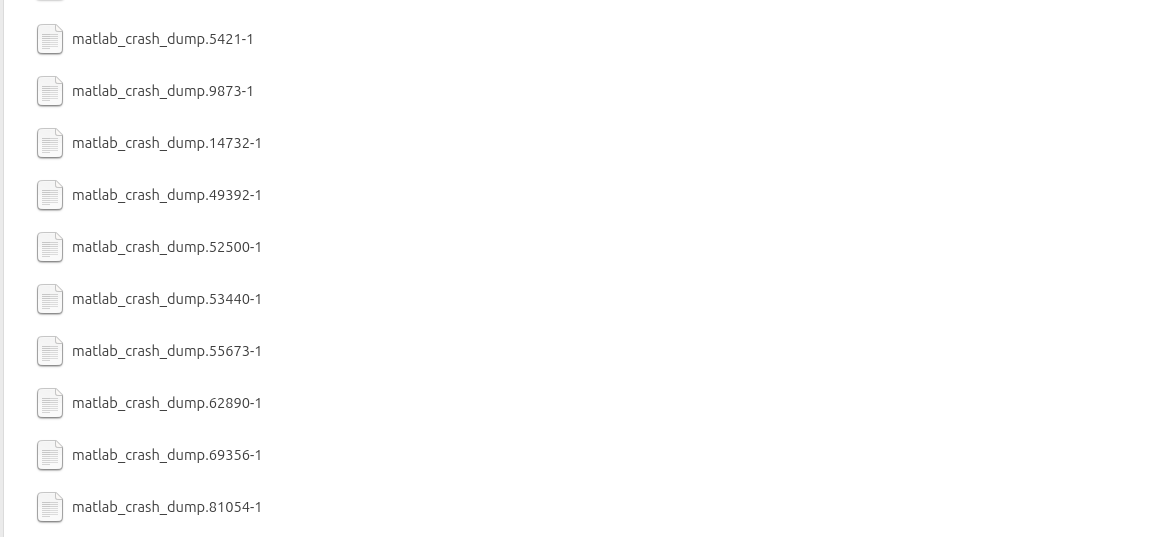
\includegraphics[width=0.75\textwidth]{run_fail.png}
  \end{figure}

\end{frame}

% ════════════════════════════
\begin{frame}{运行结果文件夹}

  \begin{columns}[T]
    \column{0.5\textwidth}
    \centering
    
\includegraphics[width=\textwidth]{result_dir1.png}

    \column{0.5\textwidth}
    \centering
    
\includegraphics[width=\textwidth]{result_dir2.png}
  \end{columns}

\end{frame}
% ════════════════════════════
\begin{frame}{解决方案}

  \begin{itemize}
    \item AI 辅助优化 \texttt{exporthist.m}。
    \item 扩大虚拟机内存与 swap 空间
    \item 串行改为 8 核并行池（\texttt{parpool}）
    \item 将 benchmark 的 \texttt{maxdim} 从 20 降至 10
    \item 关闭图形化界面改为纯命令行运行。
  \end{itemize}

\end{frame}

% ════════════════════════════
\begin{frame}{实验结果}

  \textbf{Rosenbrock} —— 四种约束条件下均收敛至合理最优值

  \vspace{0.3em}
  \textbf{S2MPJ 精度对比} —— double 与 single 存在可观测差距，double 与 quadruple 性能曲线基本重合

  \vspace{0.5em}
  \begin{columns}[T]
    \column{0.5\textwidth}
    \centering
    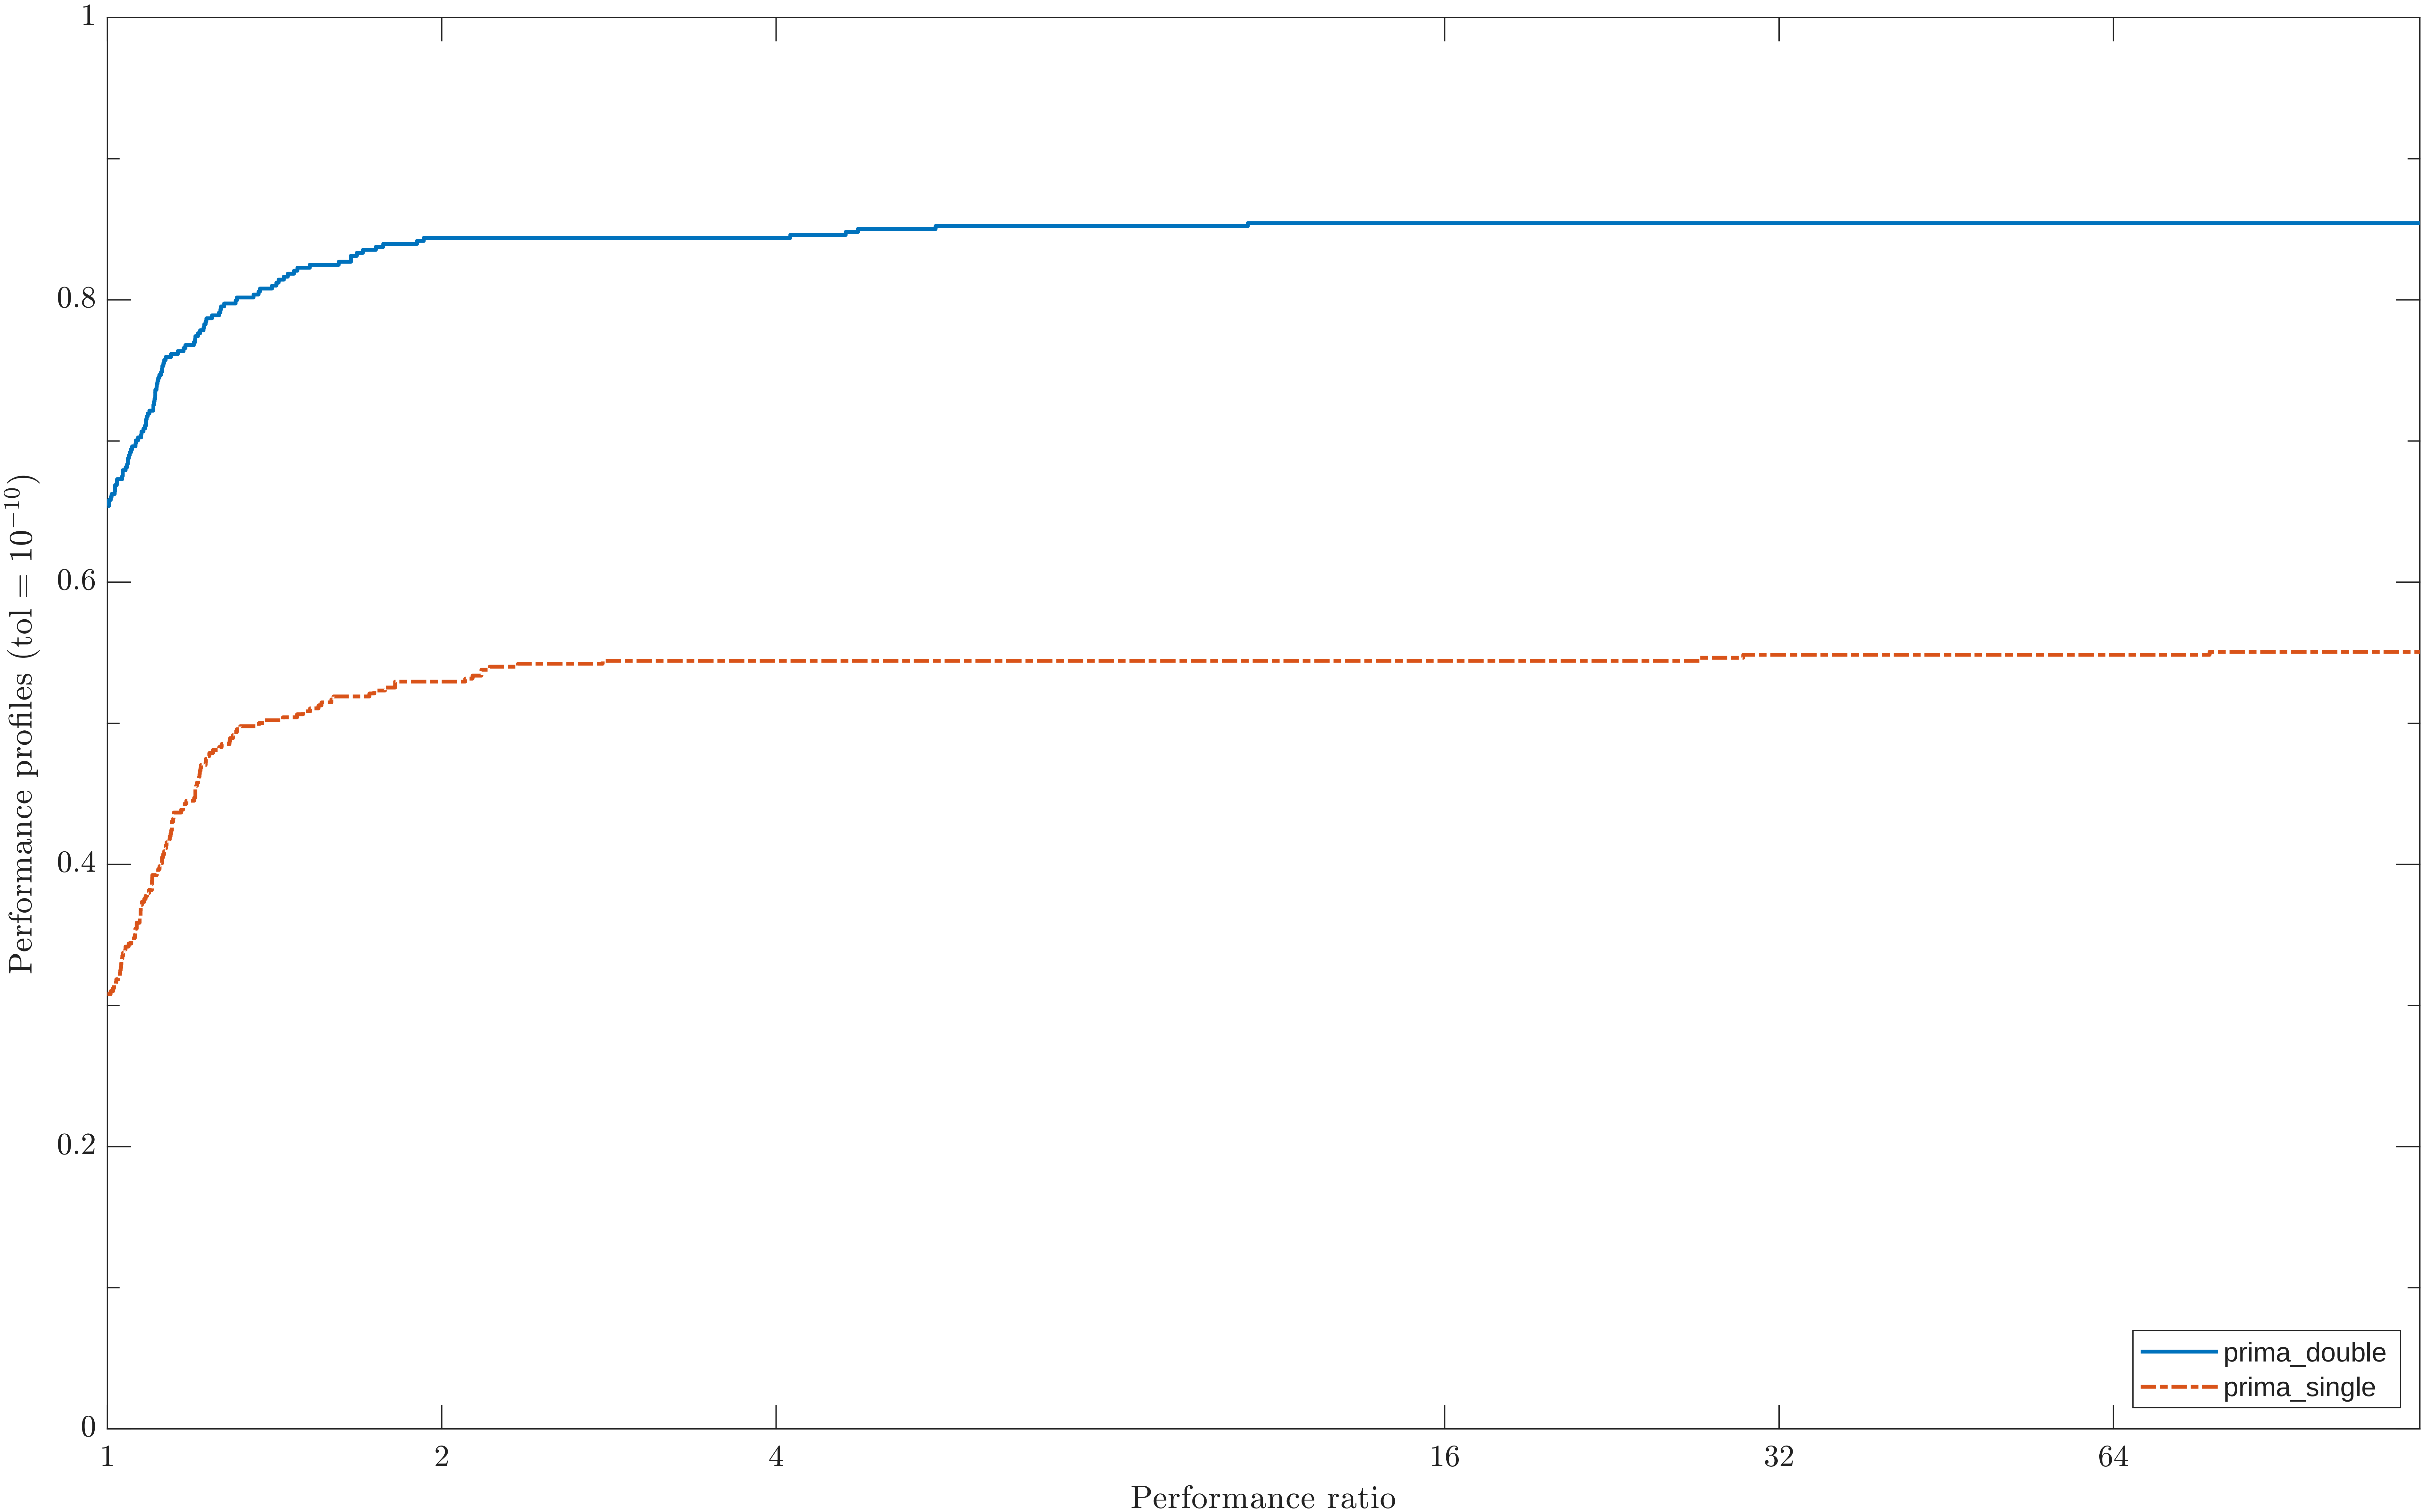
\includegraphics[width=\textwidth]{perf_plain_ds.png}

    {\small plain}

    \column{0.5\textwidth}
    \centering
    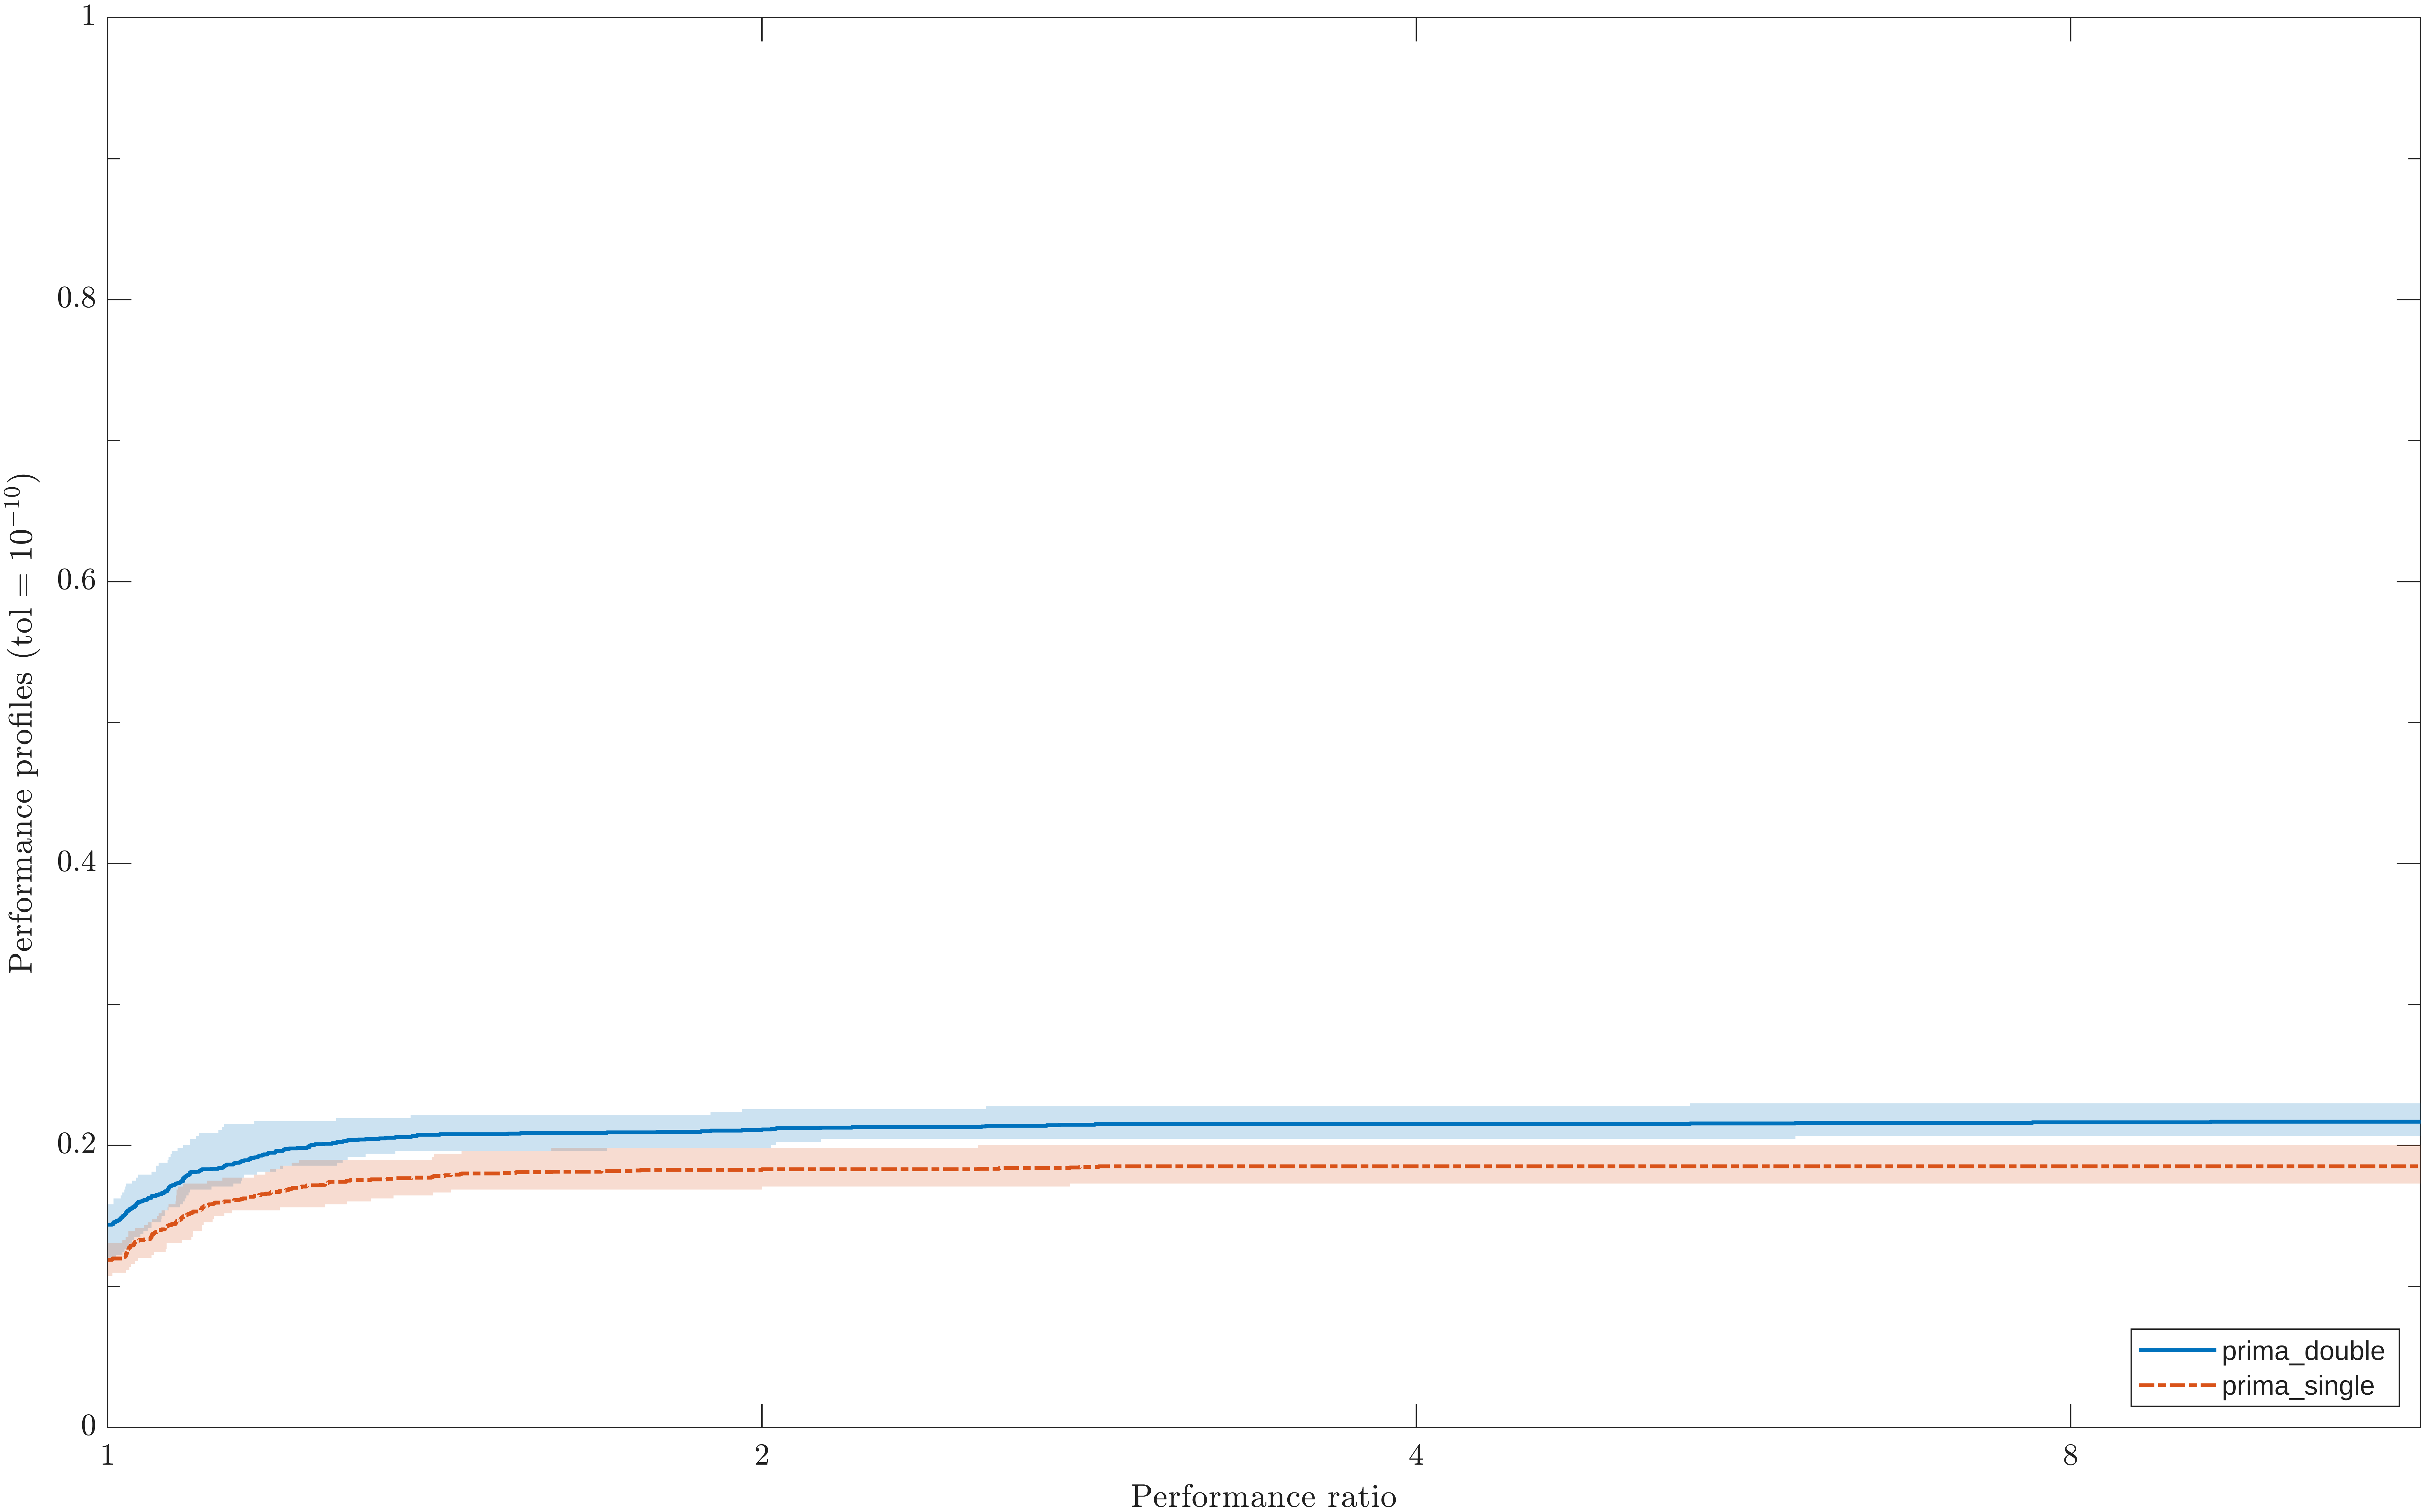
\includegraphics[width=\textwidth]{perf_noisy_ds.png}

    {\small noisy}
  \end{columns}

\end{frame}

\end{document}
